\chapter{Analyse SXCS}\label{lcs_analysis:cha}

\begin{table}[ht]
\caption{Vergleich ``Intelligent (Open)'' und ``Intelligent (Hide)'' (8 Agenten, S�ulenszenario)}
\centering
\begin{tabular}{c c c}
\hline\hline
Algorithmus & Abdeckung & Qualit�t \\ [1ex]
\hline
``Intelligent (Open)'' \\ [1ex]
\hline
Zuf�llige Bewegung     & 72.55\% & 11.58\% \\
XCS                    & 71.35\% & 13.98\% \\
SXCS                   & 72.10\% & 13.50\% \\ [1ex]
\hline
``Intelligent (Hide)'' \\ [1ex]
\hline
Zuf�llige Bewegung     & 72.56\% & 11.78\% \\
XCS                    & 71.33\% & 14.27\% \\
SXCS                   & 72.05\% & 13.90\% \\ [1ex]
\hline
\end{tabular}
\label{table:intelligent_open_hide_pillar}
\end{table}


\begin{table}[ht]
\caption{Vergleich ``Intelligent (Open)'' und ``Intelligent (Hide)'' (8 Agenten, S�ulenszenario)}
\centering
\begin{tabular}{c c c}
\hline\hline
Algorithmus & Abdeckung & Qualit�t \\ [1ex]
\hline
``Intelligent (Open)'' \\ [1ex]
\hline
Zuf�llige Bewegung     & 72.55\% & 11.58\% \\
XCS                    & 71.35\% & 13.98\% \\
SXCS                   & 72.10\% & 13.50\% \\ [1ex]
\hline
``Intelligent (Hide)'' \\ [1ex]
\hline
Zuf�llige Bewegung     & 72.56\% & 11.78\% \\
XCS                    & 71.33\% & 14.27\% \\
SXCS                   & 72.05\% & 13.90\% \\ [1ex]
\hline
\end{tabular}
\label{table:intelligent_open_hide_pillar}
\end{table}


TODO 
%if((sensor_goal[2*i])) {//  && (!sensor_agent[2*i+1])) { vergleichen. Ohne Sensoragent minimal schlechter

TODO auch sich langsam bewegende analysieren!
Und auch stehenbleibende : z.B. im Raumszenario.

Geschwindigkeit 2 problematisch, Geschwindigkeit 1 ok?

TODO classifier ausgeben 

\section{Vergleich unterschiedlicher Geschwindigkeiten des Zielobjekts}

In Abbildung~\ref{goal_agent_speed:fig} ist ein Vergleich der unterschiedlicher Geschwindigkeiten des Zielobjekts dargestellt. XCS (mit 500 Schritten) macht bei keiner Geschwindigkeit Lernfortschritte, die Qualit�t pendelt zwischen 31.69\% und 33.40\%, also in etwa identisch mit der zuf�lligen Bewegung. Die SXCS Implementierung scheint dagegen die geringere Geschwindigkeit ausgenutzt zu haben und ist dadurch in der Lage das Zielobjekt besser zu verfolgen. Mit 500 Schritten ist die Qualit�t abnehmend von 39.64\% (Geschwindigkeit 1.0) bis 35.96\% (Geschwindigkeit 2.0), im Fall mit 2000 Schritten erh�ht sich dieser Bereich leicht auf 40.15\% bis 37.71\%.\\
Auch bei den Heuristiken zeichnet sich ein klares Bild ab, bei niedrigen Geschwindigkeiten ist die Ausbreitung der Agenten auf dem Feld (intelligente Heuristik) weniger wichtig als die konstante Verfolgung des Zielobjekts, w�hrend bei h�heren Geschwindigkeiten die Verteilung auf dem Feld wichtiger wird.

\begin{figure}[htbp]
\centerline{	
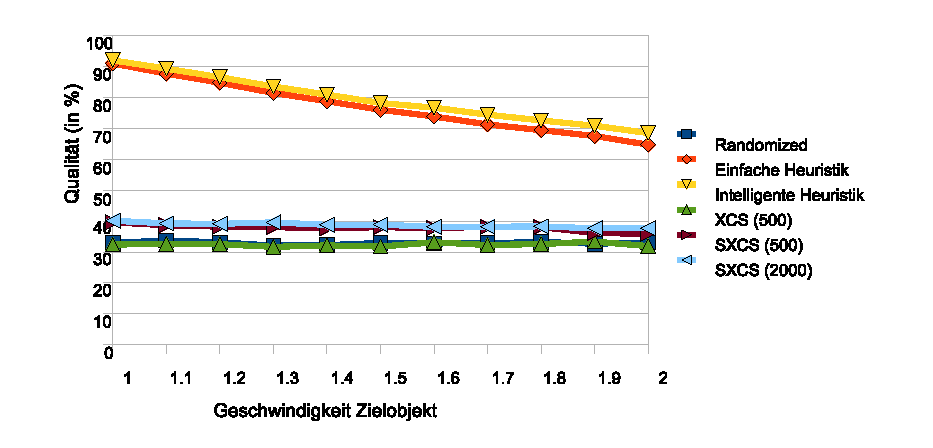
\includegraphics{goal_agent_speed.eps}
}
\caption[Vergleich der Qualit�ten verschiedener Algorithmen bez�glich der Geschwindigkeit des Zielobjekts] {Vergleich der Qualit�ten verschiedener Algorithmen bez�glich der Geschwindigkeit des Zielobjekts}
\label{goal_agent_speed:fig}
\end{figure}

\begin{verbatim}
Bester Agent nach 20000 Schritten (Zielgeschwindigkeit 2.0, SXCS, 2000 Schritte)

#0######.###0#0##.#0#0###0-S : [Fi: 0.38] [Ex: 00450.0] [Pr: 0.74] [PE: 0.38]
....
TODO
\end{verbatim}


\section{Zusammenfassung der bisherigen Erkenntnisse}

 Algorithmen mit Ergebnissen die unter dem des zuf�lligen Algorithmus liegt, sind unbrauchbar und nicht vergleichbar. ``Verbesserungen'', die die Qualit�t des Algorithmus n�her an das Ergebnis des zuf�lligen Algorithmus bringen, sind in Wirklichkeit Ver�nderungen, die den Algorithmus eher zuf�llige Entscheidungen treffen lassen, und keine tats�chlichen Lernerfolge.

SXCS sehr gut bei NO DIRECTION CHANGE und speed 1!


nicht geschafft: Pillar, one direction change, speed 2, XCS ...besser... weil zuf�lliger


\section{Standard XCS Multistepverfahren}

\subsection{SXCS und Heuristiken}

erst multistep... mit random vergleichen

In allen Tests erreichten die Heuristiken deutlich bessere Ergebnisse. Diesen Nachteil hat sich LCS in diesen Szenarien durch deutlich �berlegene Flexibilit�t erkauft
Ein Gro�teil der eingehenden Informationen ist f�r die Auswertung nicht relevant und lokale Information ist zu ungenau.
Bei einer komplexeren Implementierung mit Distanzen

Insbesondere der Vergleich mit dem intelligenten Agenten, der anderen Agenten ausweicht, zeigt, dass die LCS Agenten unm�glich ein solches globales Ziel erreichen k�nnen, es ist also kein emergentes Verhalten zu beobachten. Dies ist dadurch zu begr�nden, dass bei der Berechnung des Rewards keine Information au�er der eigenen, lokalen Information 

der Abstand zu anderen Agenten nicht Teil der Berechnung des Rewards ist, noch gibt keine eingebaute Heuristik. Man k�nnte zwar 


TODO statistical value:Error in predictions!

\subsection{Vergleich Multistep / LCS}

Szenarien, Parameter.

\subsection{Test der verschiedenen Exploration-Modi}


Prediction Error sehr hoch, da dynamisches 
